\documentclass{standalone}
\usepackage{tikz}
\usetikzlibrary{patterns, arrows.meta}
\begin{document}
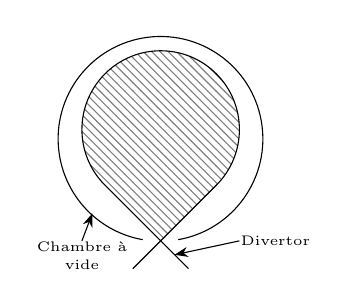
\begin{tikzpicture}

	\def\y_xpoint{0}
	\def\angle{45}
	
	\pgfmathparse{cos(\angle)}
	\let\cos=\pgfmathresult

	\pgfmathparse{sin(\angle)}
	\let\sin=\pgfmathresult

	\fill[pattern=north west lines, pattern color=gray]
		(0, \y_xpoint) -- (\cos, \sin) -- (\cos, \sin)	arc[start angle=-\angle, end angle=180+\angle, x radius=1, y radius=1]
    -- (0, \y_xpoint);
    
    \draw
		(0, \y_xpoint) -- (\cos, \sin) -- (\cos, \sin)	arc[start angle=-\angle, end angle=180+\angle, x radius=1, y radius=1]
    -- (0, \y_xpoint);
    
    \draw (0, \y_xpoint) -- (\cos/2, \y_xpoint-\sin/2);
    
    \draw (0, \y_xpoint) -- (-\cos/2, \y_xpoint-\sin/2);
    
    \draw[{Stealth}-]  (\cos/4, \y_xpoint-\sin/4) -- (1, 0) node[right=-3pt, align=center] {\tiny\shortstack{Divertor}};
    
    \def\angle{-80}
	
	\pgfmathparse{cos(\angle)}
	\let\cos=\pgfmathresult

	\pgfmathparse{sin(\angle)}
	\let\sin=\pgfmathresult
    
    \draw (\cos+0.05, \sin+1)	arc[start angle=\angle, end angle=180-\angle, x radius=1.3, y radius=1.3];
    
    \draw[{Stealth}-] (-\cos*5, \cos*2) -- (-1, 0) node[below=-3pt, align=center] {\tiny\shortstack{Chambre à\\ vide}};

\end{tikzpicture}
\end{document}
